\chapter*{Mengubah String ke Integer dan proses Aritmatika}

\par
didalam python tipe data dapat diubah dan dilakukan proses aritmatika didalamnya, contohnya sebagai berikut.

\begin{enumerate}
	\item buka spyder dan ketik kode sebagai berikut untuk mengubah dari string ke int.
	\begin{figure} [h]
	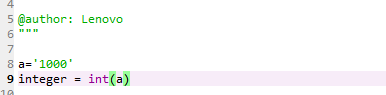
\includegraphics[width=12cm]{string/str1.png}
	\centering
	\end{figure}
	
	\item setelah itu maka ketika integer di print akan menghasilkan sebagai berikut
	\begin{figure} [h]
	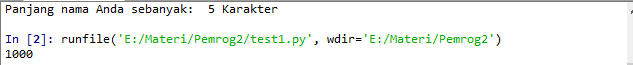
\includegraphics[width=12cm]{string/str2.png}
	\centering
	\end{figure}
	
	\item Setelah tipe data diubah, dapat langsung dikombinasikan dengan proses aritmatika
	
	\item untuk melakukan proses aritmatika maka dapat dilakukan dengan menuliskan kode sebagai berikut
	\begin{figure} [h]
	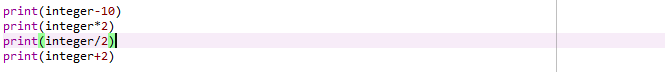
\includegraphics[width=12cm]{string/str3.png}
	\centering
	\end{figure}
	
	
	\item setelah menuliskan kode jangan lupa menuliskan perintah print
	
	\item setelah itu silahkan menjalankan script yang sudah dibuat
	

	
	

	\end{enumerate}
	
	

